%--------------------------------------------------------------------
%
%Mustervorlage fuer eine Aufgabe
%
%--------------------------------------------------------------------
%
%Ueberschreiben der automatisch erzeugten Aufgabennummer
%Die folgende Aufgabennummer ergibt sich aus dem Stand des
%Z�hlers + 1
%\setcounter{chapter}{0}
%
\chapter{Results and Future Work}\label{chap:results}
%
%
%
In the previous chapters, different components of the project have been discussed. After setting up the ROS system on the computer, the laser scanner was put into operation, and the robot was built. Then several localization algorithms were used and tested. Lastly, the control was implemented, and the whole system was integrated all together. As explained before, the robot must follow a pre-defined line. In this chapter, the results of the control algorithm will be discussed. Finally, improvements and future work will be discussed.

\section{Control Results}
 

As explained before, the robot follows a given line, which can be described with equation \ref{eq14}. In order to test the control algorithm, three different equations will be used. These equations are:

\begin{equation}\label{eq20}
y + x = 0 
\end{equation}
\begin{equation}\label{eq21}
y - 0.5 = 0 
\end{equation}
\begin{equation}\label{eq22}
x + 0.5 = 0 
\end{equation}

Each equation corresponds to a different line. Equation \ref{eq22} corresponds to a straight line that is parallel to the Y-Axis. This line will be labeled as Path A. Path B is a straight line that is parallel to the X-Axis, which corresponds to equation \ref{eq21}. Lastly, Path C, which is a sloped line that corresponds to equation \ref{eq20}. For each equation, different initial poses will be tested. The poses are noted as following $(x,y,\theta)$, where $x$ and $y$ correspond to the position of the robot, and $\theta$ corresponds to the orientation of the robot. The different pathes are plotted in runtime using MatplotLib library.\\

\textbf{Path A:}\\
As displayed in figure \ref{fig:fig15}, two different initial poses have been considered. The first initial pose is $(-0,1.15,180�)$. The second initial pose is $(-0,1.15,180�)$. In both cases, the robot successfully controlled its motion to follow the given line.

\begin{figure}[ht]
\begin{subfigure}[c]{1\textwidth}
  \centering
  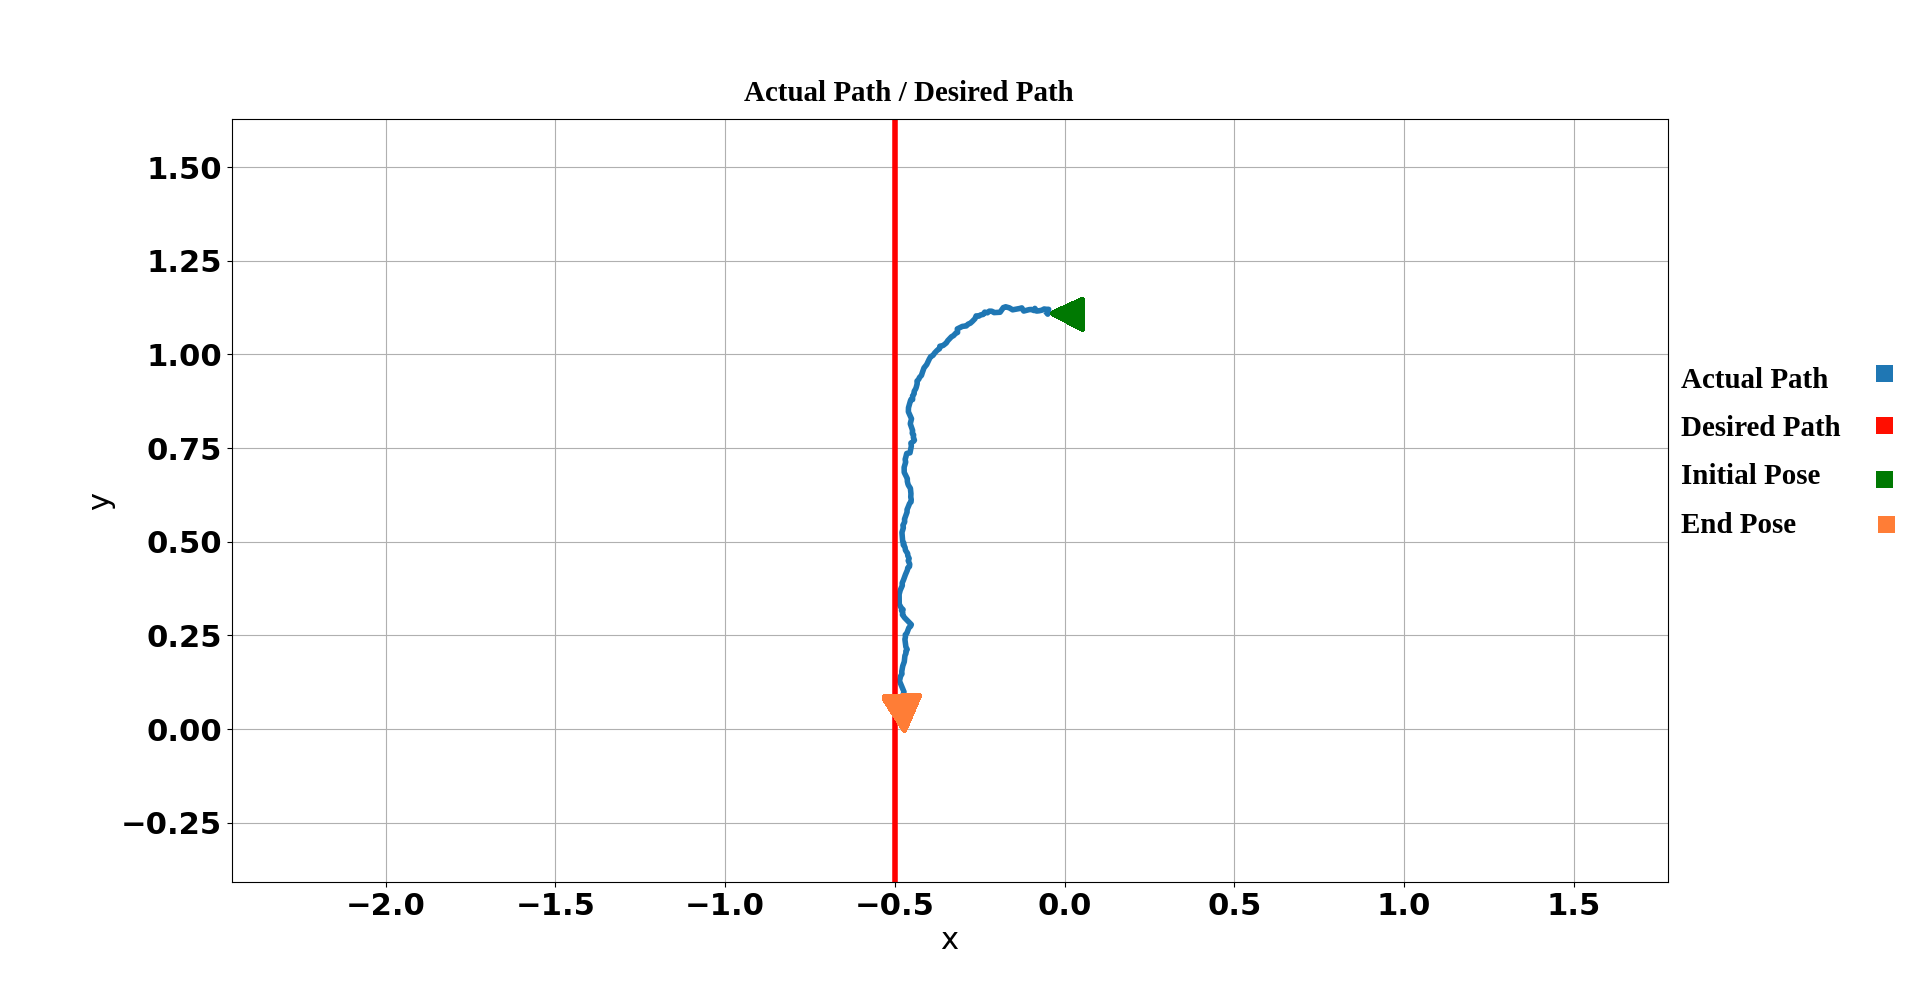
\includegraphics[width=1\linewidth]{./Bilder/Figure_1A.png}
  \caption{First initial pose}
  \label{fig15:sfig1}
\end{subfigure}%

\hspace*{\fill}%          % empty line absolutely necessary!
\begin{subfigure}[c]{1\textwidth}
  \centering
  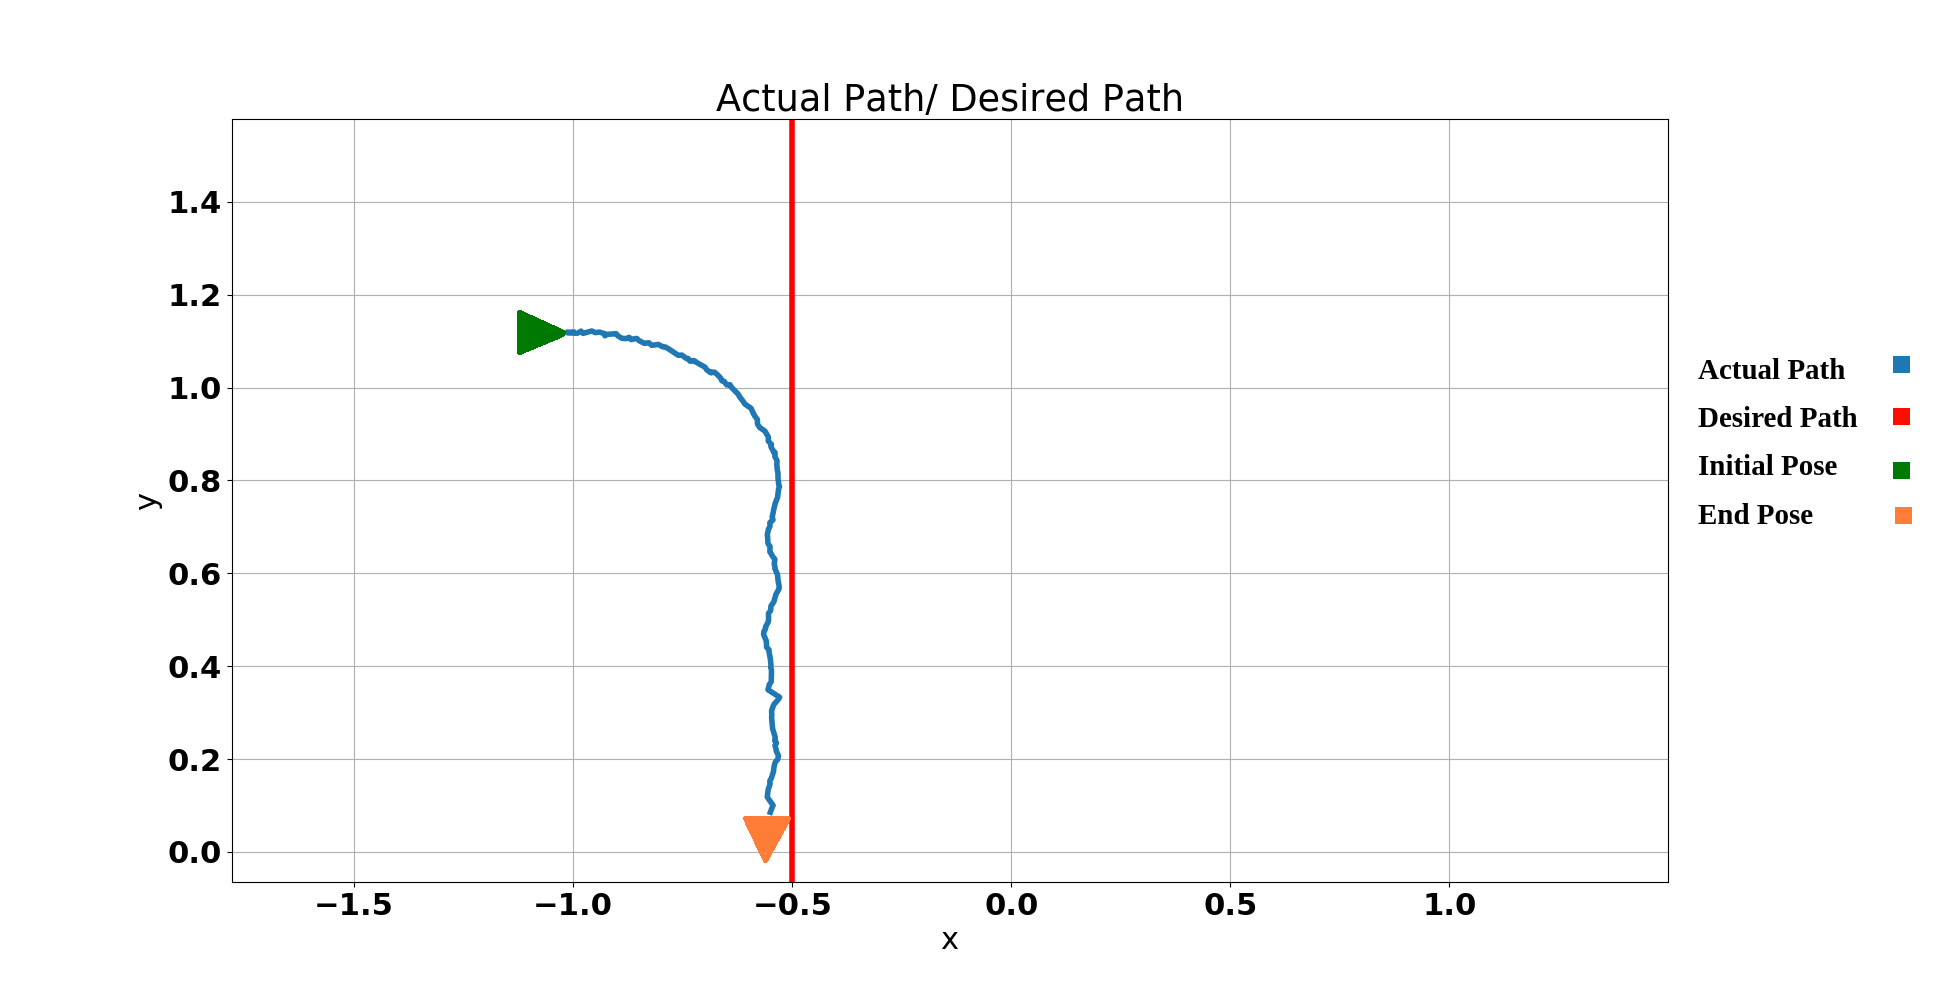
\includegraphics[width=1\linewidth]{./Bilder/Figure_1B.png}
  \caption{Second initial pose} 
  \label{fig15:sfig2}
\end{subfigure}
\caption{Robot motion control: Path A.}
\label{fig:fig15}
\end{figure}
 
\textbf{Path B:}\\
The same as in Path A, two different initial poses have been considered. The first initial pose is $(-0.21,0.05,90�)$. The second initial pose is $(-0.05,1.1,315�)$. In both cases, the robot successfully controlled its motion to follow the given line. The motion of the robot in both cases is displayed in figure \ref{fig:fig16}


\begin{figure}[ht]
\begin{subfigure}[c]{1\textwidth}
  \centering
  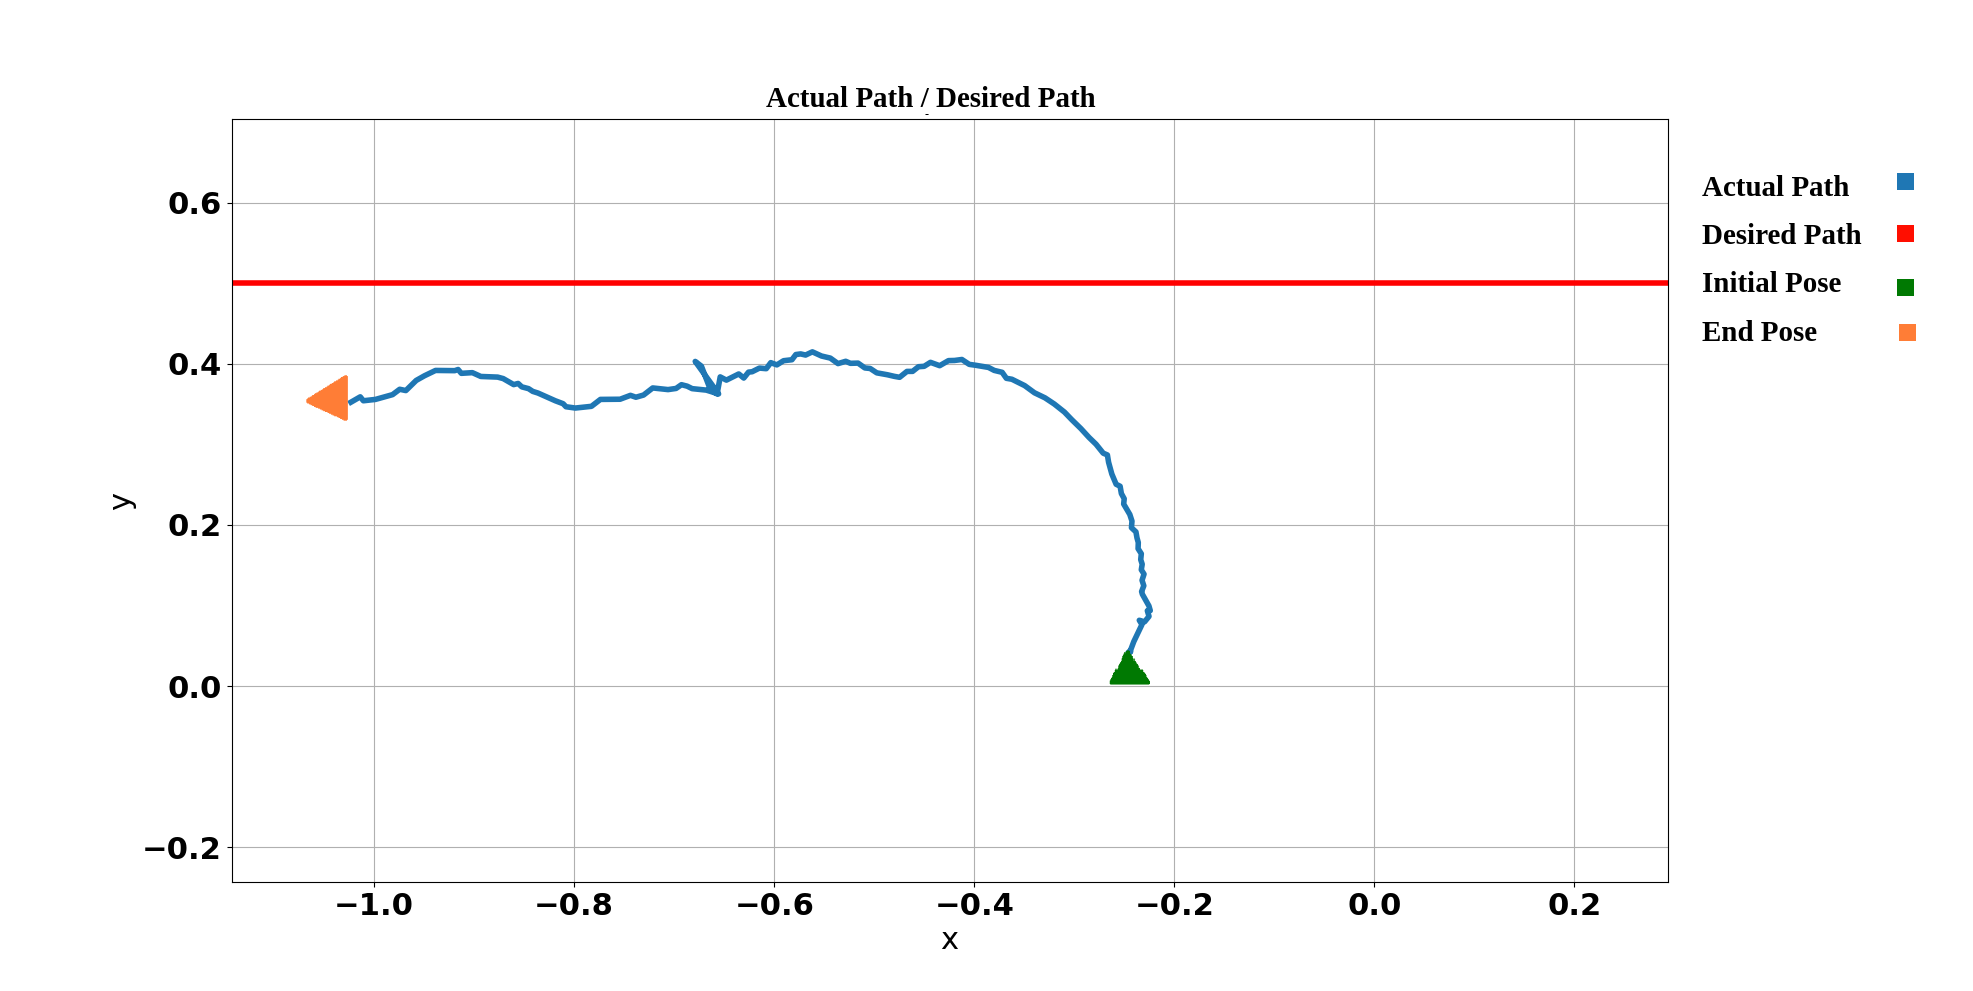
\includegraphics[width=1\linewidth]{./Bilder/Figure_2A.png}
  \caption{First initial pose}
  \label{fig16:sfig1}
\end{subfigure}%

\hspace*{\fill}%          % empty line absolutely necessary!

\begin{subfigure}[c]{1\textwidth}
  \centering
  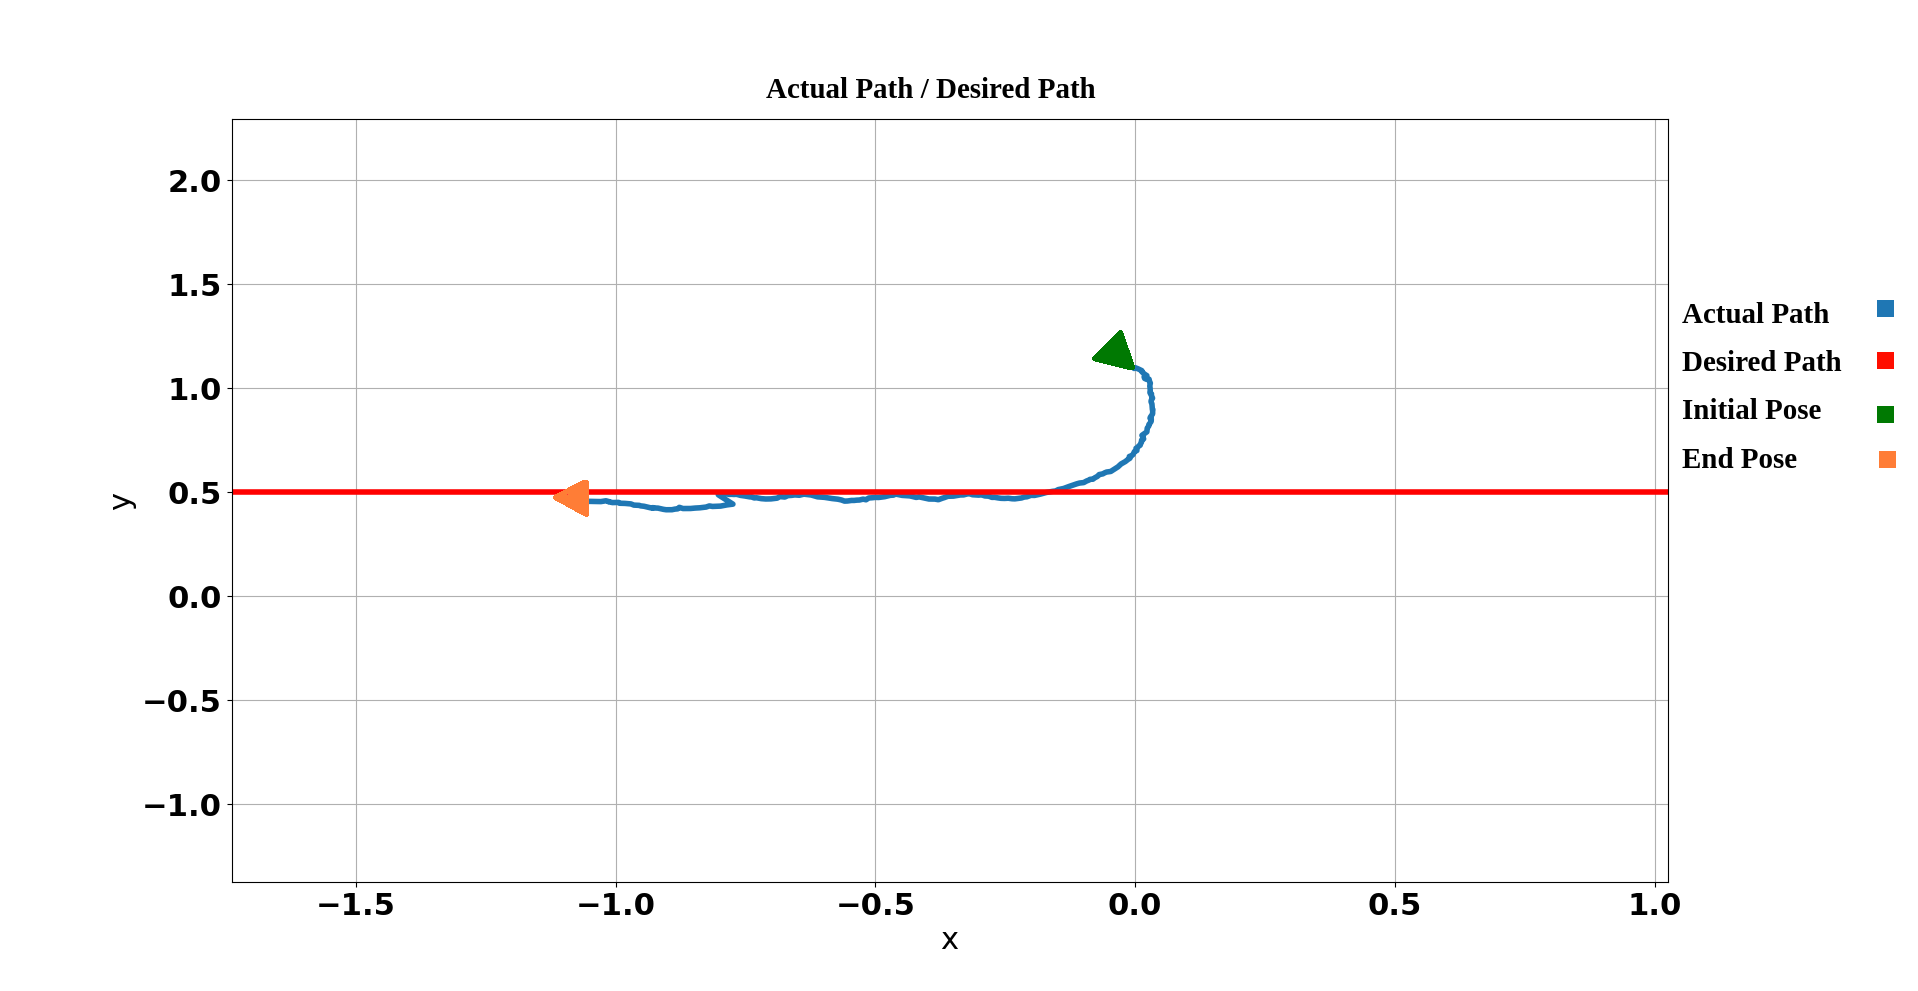
\includegraphics[width=1\linewidth]{./Bilder/Figure_2B.png}
  \caption{Second initial pose} 
  \label{fig16:sfig2}
\end{subfigure}
\caption{Robot motion control: Path B.}
\label{fig:fig16}
\end{figure}
 

\textbf{Path C:}\\
As displayed in \ref{fig17}, the initial pose of the robot is $(-0.25,0,90�)$. The robot follows the given line.
\begin{figure}[ht]
	\centering
	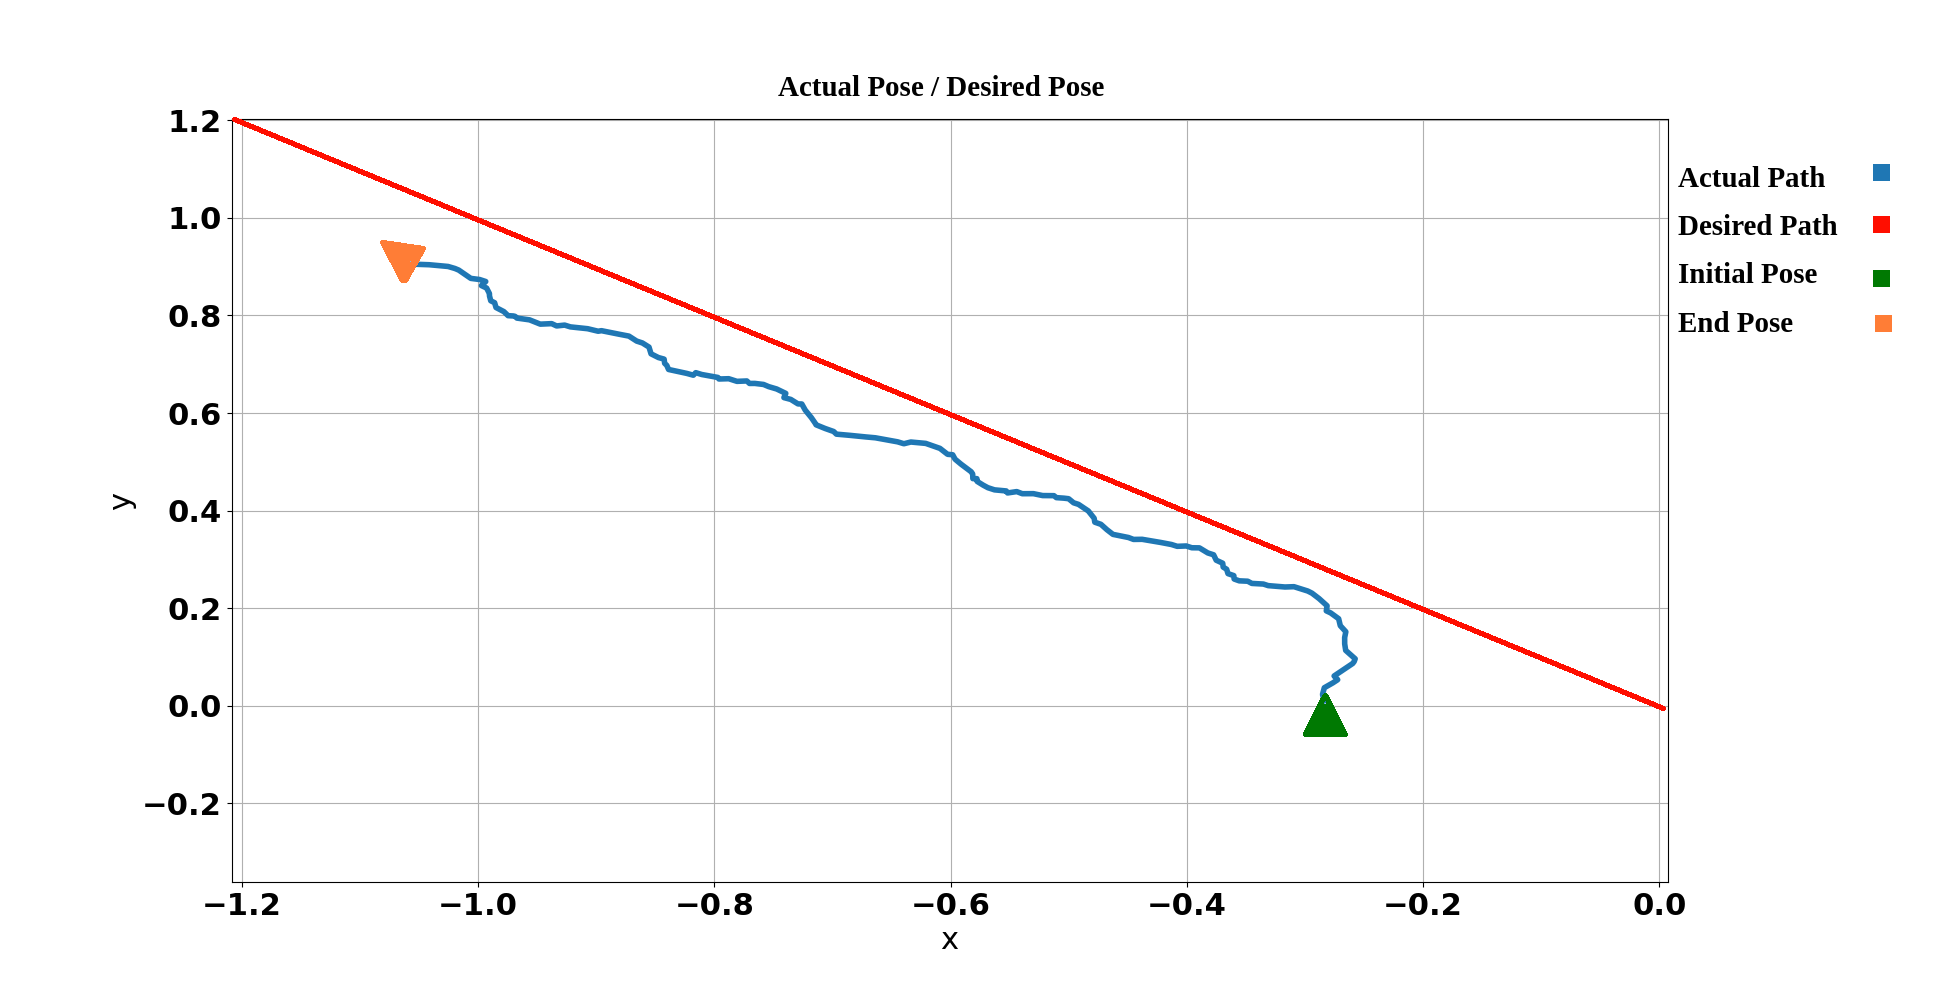
\includegraphics[width = 1\textwidth]{./Bilder/Figure_3A.png}
	\caption{Robot motion control: Path C}
	\label{fig17}
\end{figure}\\


As displayed in the previous figures, the robot was able to follow the pre-defined lines as expected. However, since two different proportional controllers are used, there is an offset to the given path. This offset occurs due to the inaccuracy of the proportional controller. Another problem that can be observed is the oscillations of the robot motion after the distance is minimized. This problem can be solved by adding a hysteresis.\\

Although the performance of the control algorithm was not ideal, this approach provides several advantages. The most important advantage is the extensibility of the software. In other words, other nodes and components can be added easily to the software to improve the results or even to add new features. Another advantage of this approach is the reusability of the nodes. The control algorithm node, for example, can be used to any other robot. The presented results show the feasibility.
An optimization of the control system will improve the behaviour considerably, but unfortunately could not be tackled in the time frame of this work.


\section{Future Work} 

As explained before, since this project based on ROS, other components can be added and integrated into the software. Thus, many different applications and ideas can be added. The next step is to add other control algorithms, i.e., to let the robot follow a trajectory or to make it move to a specific pose. Many of these control algorithms are explained in \cite{corke_robotics_2017}. Moreover, the whole system can be simulated using Gazebo. Gazebo is a simulation tool used in the field of robotics to simulate robots.
Furthermore, the system can also be extended to contain more than one robot at the same time. 